\documentclass[11pt, titlepage]{article}

\usepackage[a4paper, margin=1in]{geometry}
\usepackage{graphicx}

\author{\textbf{The Terminal}}

\title{\textbf{Coast Capital Contractor Records Database System - Project Plan}}

\begin{document}

\maketitle

\tableofcontents

\clearpage

\section{Overview}

Coast Capital is a Canadian credit union that offers a variety of services to customers such as banking, investments and lending. They use contractors for various needs to aid their own employees when project demands are high. Currently Coast Capital uses excel spreadsheets to manage and capture data relating to their contractors. The process of using spreadsheets can be unorganized and is not very straightforward for a new user. Even though it is simple, it takes too long to update and involves a lot of manual work. Furthermore, the data is not captured in their HR system and it is never guaranteed that various spreadsheets will be in sync or have the most up to date data as any individual working on a spreadsheet will have a different copy due to spreadsheets being an offline tool. The aim of our project is to simplify the system Coast Capital uses for capturing contractor data and hopefully to move them away from using spreadsheets to using our application.

The system our team (�The Terminal�) will be building will be an online web application designed for ease of use and powerful data analysis.  The application aims to make it a straightforward process to add, edit, and visualize contractor data. Our application will be easy to learn for new users such that there is not a long ramp-up period for using it in comparison to using excel spreadsheets. Furthermore, since our application is an online web tool, all the contractor data within it will always be the most up to date data available so no two users are viewing different data.  

Our team will be using various aspects of agile to ensure each member of our group knows what the other members of the group are doing at all times. To accomplish that, we will be having biweekly meetings to give updates on our individual progress to each of the team members.  This scrum type methodology ensures that we can address concerns with individual members before they are out of control. Moreover, we will be using Test Driven Development for our development process so that our application is constantly being tested from day 1 of development. Effectively this means our application will be less error prone and will contain fewer bugs and that the bugs it does contain will be found early on in the development process so we can address them sooner rather than later. We will also have cross-functional teams as we have divided our team into smaller teams in charge of handling different aspects of the project.


\section{Estimated Schedule}

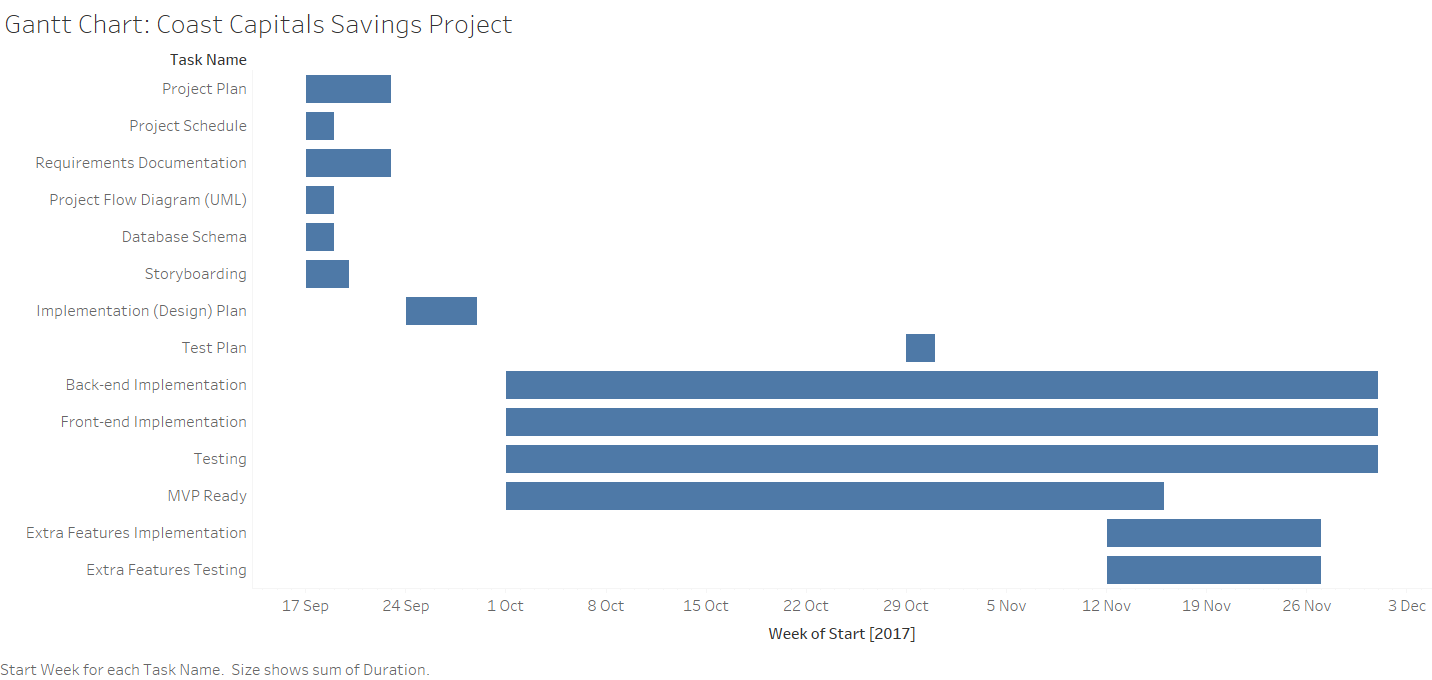
\includegraphics[width=1.0\textwidth]{gantt}

The Gantt chart above shows the breakdown of the tasks we intend to complete (or have already completed). Both the start and end date are indicated, and so is the intended duration of each segment of the project. 

The critical paths are the planning stages, primarily finishing requirements documentation. Following that, the next critical path is creating the design plan which we would then follow when actually implementing that design. This includes database design, UI design, and figuring out all the connections in between. As we are using the Agile method of test driven development (explained previously in more detail), it has not been highlighted as a critical path, as it is something that will be ongoing alongside the coding part of the project.

\section{Resource Plan}

\subsection{Overview}

Our team has decided to follow the Agile philosophy and have divided ourselves into 4 cross-functional teams, each of which will work on a separate component.

\subsection{Roles and Responsibilities}

\begin{enumerate}
    \item Anushka will be in charge of UI/UX design.
    \item Shrey will be working on UI/UX design implementation which would include integrating all the technologies required for all the data visualization requirements.
    \item Maia will be responsible for implementing the callbacks from frontend to backend and making sure the data communication between them is functioning properly
    \item Vaastav and Stephen will be working on implementing and adding functionality for maintaining the SQL database as well as implementing handler functions for data communication with the frontend. We will be working closely with Maia in completing this.
    \item Vaastav will be the Overall Project Manager with Anushka assisting him.
\end{enumerate}

\subsection{Costs}

\begin{enumerate}

    \item We will be using an AWS server for deployment of this system and this system will be available under the BSD 3-clause license.There are some costs associated with hosting our web application on an AWS server, however the first year of an AWS membership is free so these costs will not be incurred up front. The cost of hosting on AWS is dependent on how much data is flowing through the system and how heavily the system is being used. Currently only one employee at Coast Capital maintains the contractor records, extrapolating from that our system will not have very heavy traffic so the cost associated with usage should be fairly low. Furthermore, since an AWS server automatically scales capacity based on usage there will only be costs based on how much the system is actually being used, helping prevent paying for unused capacity. 
    \item We will also be using Travis-CI for doing automated builds for all pull requests so that we can keep track of issues and errors. This will have no monetary cost associated with it.

\end{enumerate}

\section{Design Plan}

\subsection{Front End Design}

Coast Capital's current UI can be complicated which makes it difficult to learn for employees who do not use it regularly. Our design approach aims to make the UI learnable and efficient.

\begin{enumerate}
    \item Their system of making pivot tables is very efficient and with some adjustments, it should become easy to learn as well.
    \item  We will be making a paper prototype of the website to visualize our whole design before implementing it. It will have all the basic functionalities including safety prompts, which will ensure that we eliminate all UI risks in the system. 
\end{enumerate}

\subsection{Database Design}

Coast Capital currently saves a lot of information and data in their contractor records. Our goal is to design a database schema that represents this information and data in an organized and easily accessible fashion. In order to achieve this we will be making an Entity-Relationship (ER) diagram that will help us understand and realise what all information needs to be saved and what all tables we need to store in the database in order to represent this information in an efficient manner.

\subsection{Overall System Design}

For designing the system, we will be defining the architecture, the modules, interfaces, data and the communication process between the frontend and backend server to meet the technical as well as non-technical requirements of the user. Sample data has already been provided to us by Coast Capital Savings. In addition, we will also generate some mock data for testing our system thoroughly. We will be using Java and SQL for implementing the backend and Javascript, HTML and CSS for implementing the frontend and callbacks to the server. We will also be creating the a UML diagram to highlight how communication of data will take place and how it will be used throughout the system. This will essentially behave like a call graph for the system.

\section{Development Plan}

\subsection{Module Based Development}

\begin{enumerate}
    \item Our team has identified that the system will have the following 3 major layers
            \begin{enumerate}
                \item \textbf{Database and Server Layer} : Responsible for creating, maintaining and updating tables in the database.
                \item \textbf{Communications Layer} : Responsible for verifying input data for correctness, sending data to the backend and receiving data from the backend.
                \item \textbf{User Layer} : Responsible for allowing the users to add, edit and view data in the database as well as generating reports.
            \end{enumerate}
    \item Each layer will have different modules and our approach will be centered towards completing these modules for functionality in order to progress whilst building our system. Each module will correspond to a big feature in the system.
\end{enumerate}

\subsection{Documentation Plan}

\begin{enumerate}
    \item We will be continuously documenting our code in Javadoc style so that Javadoc can be produced which will help in aiding and understanding the code.
    \item We will also produce a deployment document which will highlight all the steps required to deploy this system on a server like an AWS server. This will essentially be the steps we take to deploy the system on an AWS server for the testing phase.
    \item We also plan on making a tutorial for employees who enter the website for the first time.
\end{enumerate}

\section{Testing Plan}

\subsection{Overview}

Our team has decided to adopt the Agile philosophy of Test Driven Development for this project and thus we will be testing from the very first day we start writing code. However, our testing will be broken into multiple phases.

\subsection{Unit Testing}

Before adding any new function to be used for a featured, unit tests will be written to test individual aspects of the function and the function itself. The unit tests will capture all the edge cases and basic individual functionality of the function. We will be JUnit as the testing framework for implementing our unit tests. This will be done throughout the development phase. We will be using Mocha as our testing framework for testing JavaScript Code.

\subsection{Integration Testing}

As mentioned before, we would be breaking the project down into multiple components and modules so it is important to test that these modules combine together to work correctly. We will be writing automated integration tests to test this functionality although some of the working modules might have to be tested for integration manually.

\subsection{Front-End Testing}

As the system we are making is a web-browser based system, we have decided to have a test suite for testing our front end code that basically tests the functionality of the forms our website will be using, the way data is received from and sent to the database and the way the data is manipulated and used. This is to ensure that the communication lines between the backend database server and the frontend browser are properly functioning and the data being received is being correctly used. We will be achieving this by using Selenium for automated testing.

\subsection{Cross Browser Testing}

The technical requirements of the project require that the system must be supported on IE11 and Firefox as these two browsers are the more widely used browsers throughout Coast Capital. So, we will be testing our system on both IE11 and Firefox by a combination of automated test suites with Selenium and manual visual testing.

\subsection{System Integration Testing}

We will do system integration testing once we have a completed version of the web-based database system to ensure that all the requirements and specifications are captured and working correctly from an overall system point of view. Our System Integration Tests will behave as our technical acceptance tests. This will most likely be done via manual testing.

\subsection{User Acceptance Testing}

In addition to System Integration Testing, we will also be doing User Acceptance Testing to ensure that we are not only meeting the technical requirements but also actually meeting the needs of the Users and that the system we have developed is an easy to use and manipulate system from the point of view of the user. Just like System Integration Testing, this will also be done manually.

\section{Deployment Plan}

Our current plan is to deploy our system on an AWS server and we will be doing this once we have the database completely configured and some basic UI functionality with callbacks to the backend server implemented.

\end{document}
